% arara: pdflatex
% arara: bibtex
% arara: pdflatex
% arara: pdflatex
\documentclass[journal]{IEEEtran}
\pdfoutput=1
\usepackage[pdftex]{graphicx}
\DeclareGraphicsExtensions{.eps}
\usepackage{amsmath}
\usepackage{color}

\newif\ifarxiv
%\arxivtrue
\arxivfalse

% IF FOR ARXIV, PUT EDL's LEGAL TEXT
\ifarxiv
  \usepackage[firstpage]{draftwatermark}
\SetWatermarkText{\shortstack{\textit{This work has been submitted to the IEEE for possible publication.}\\\textit{Copyright may be transferred without notice, after which this version may no longer be accessible.}}}
  \SetWatermarkAngle{0}
  \SetWatermarkColor{red}
  \SetWatermarkLightness{0}
  \SetWatermarkVerCenter{.5in}
  \SetWatermarkFontSize{10pt}
\fi

% revision
\usepackage[normalem]{ulem}
%\newcommand{\revisein}[1]{{{\color{red}{#1}}}}
%\newcommand{\reviseout}[1]{{\color{red}\sout{#1}}}
\newcommand{\revisein}[1]{#1}
\newcommand{\reviseout}[1]{}

%\hyphenation{communi-cations semi-conduc-tor}

% Silence warning that Text page contains only floats
%\usepackage{silence}
%\WarningFilter{latex}{Text page}


\begin{document}

\title{High Breakdown Voltage in Strained AlN/GaN/AlN Quantum Well HEMTs}

\author{Austin Hickman, Reet Chaudhuri, Samuel James Bader, Kazuki Nomoto, \IEEEmembership{Member, IEEE}, Kevin Lee, \\ Huili Grace Xing, \IEEEmembership{Senior Member, IEEE}, and Debdeep Jena, \IEEEmembership{Senior Member, IEEE}%
\thanks{
  This work was supported by Semiconductor Research Corporation (SRC) Joint University Microelectronics Program (JUMP), AFOSR (FA9550-17-1-0048), and NSF DMR (1710298). The work was performed at Cornell NanoScale Facility (NNCI member supported by NSF ECCS-1542081), and Cornell Center for Materials Research, supported by NSF MRSEC DMR-1719875. All authors are with Cornell Univeristy, Ithaca, NY 14853. Contact: alh288@cornell.edu }}

% IF FOR ARXIV, NO HEADER
\ifarxiv \else
\markboth{IEEE Electron Device Letters,~Vol.~X, No.~Y, January~2018}%
{}
\fi
% The only time the second header will appear is for the odd numbered pages
% after the title page when using the twoside option.
% 
% *** Note that you probably will NOT want to include the author's ***
% *** name in the headers of peer review papers.                   ***
% You can use \ifCLASSOPTIONpeerreview for conditional compilation here if
% you desire.

\maketitle

\begin{abstract}
In evaluating GaN HEMTs for high-power applications, it is crucial to consider the device-level breakdown characteristics. This work replaces the conventional AlGaN barrier and common AlGaN backbarrier with AlN, and it assesses the breakdown voltage of strained AlN/GaN/AlN quantum well HEMTs for gate-drain spacings in the range of 0.27 to 5.1 microns. Results are highlighted by a high breakdown voltage of 78 V for a gate-drain spacing of 390 nm, among the best reported for submicron-channel devices. \textcolor{red}{Additionally, small-signal RF measurements showed record performance for HEMTs on the AlN platform, with $\mathrm{f_t/f_{max}}$ = 161/70 GHz. Breakdown voltage and cutoff frequency} are benchmarked against state-of-the-art GaN HEMTs, illustrating the potential for AlN/GaN/AlN quantum well HEMTs as a future platform for high-power RF transistors.
\end{abstract}

\begin{IEEEkeywords}
  GaN, AlN, electric breakdown, power
\end{IEEEkeywords}

% For peer review papers, you can put extra information on the cover
% page as needed:
% \ifCLASSOPTIONpeerreview
% \begin{center} \bfseries EDICS Category: 3-BBND \end{center}
% \fi
%
% For peerreview papers, this IEEEtran command inserts a page break and
% creates the second title. It will be ignored for other modes.
\IEEEpeerreviewmaketitle
\section{Introduction}
\IEEEPARstart{G}{allium} nitride-based devices have emerged as the leading contender for the future of high-voltage and high-frequency electronics. GaN's wide bandgap, large critical fields, high electron mobility, and excellent thermal conductivity enable low on-resistance and high breakdown voltages in GaN high-electron mobility transistors (HEMTs). Owing to the superior electron mobility in 2D electron gas channels, GaN HEMTs can switch high voltages at speeds unachievable by other semiconductors \cite{Danilovic2011}. The electron barrier of conventional HEMTs is AlGaN on a GaN buffer. The barrier and buffer limit the carrier confinement in high-voltage applications, and moving to alloy AlGaN buffers for a back barrier in high speed applications \cite{Shinohara2010, Shinohara2011, Lee2011} introduces a low thermal conductivity layer adversely affecting the heat dissipation.

To counter these bottlenecks of the current AlGaN/GaN HEMT technology, an alternative HEMT platform based on an AlN buffer was introduced \cite{Wang2012}. This platform uses a strained GaN quantum well sandwiched between binary AlN buffer and barrier layers. The large band offset and high polarization fields of AlN with GaN provide the maximum confinement of the 2DEG, allowing for aggressive vertical and lateral scaling. The large bandgap ($\sim$6 eV) and thermal conductivity ($\sim$340 W/mK) \cite{Rounds2018} of AlN provide an unmatched combination of electrical resistivity and thermal management in the nitride regime. A consequence of the AlN buffer region is a compressively strained, pseudomorphic GaN channel, lattice matched to AlN. The result is an unstressed AlN barrier with maximized bandgap \textcolor{black}{\cite{Li2014}}, a major advantage for high-voltage applications that is unique to this heterostructure. As a bonus, the AlN platform also offers the possibility of p-channel FETs towards a nitride CMOS \cite{Li2013},\cite{Bader2018}.

Previously, we demonstrated the successful growth and fabrication of strained AlN/GaN/AlN quantum well HEMTs (QW HEMTs) \cite{Wang2012,Islam2016,Song2017}. The devices exhibited $>$ 2 A/mm drain current, and potential for high-frequency performance, with an $\mathrm{f_t}/\mathrm{f_{max}}$ of 124/20 GHz \cite{Song2017}. High-voltage properties have been previously examined for HEMTs with an AlGaN barrier \cite{Chung2010,Hemts2006}, InAlN barrier \cite{Saunier2012,Snider2012}, InAlGaN barrier \cite{Guo2013,Lee2013}, AlGaN backbarrier \cite{Shinohara2010,Shinohara2011,Shinohara2011a,Tang2015}, \textcolor{black}{InGaN backbarrier \cite{YugangZhou2005,Palacios2006}}, N-polar HEMTs \cite{Dasgupta2009,Nidhi2012,Denninghoff2012,Denninghoff2012a,Denninghoff2013,Romanczyk2018}. In this letter, we demonstrate the first studies of the off-state breakdown voltage for QW HEMTs, and we benchmark their breakdown voltage and on-resistance against the existing GaN HEMT platform.
\begin{figure}[!b]
\centering
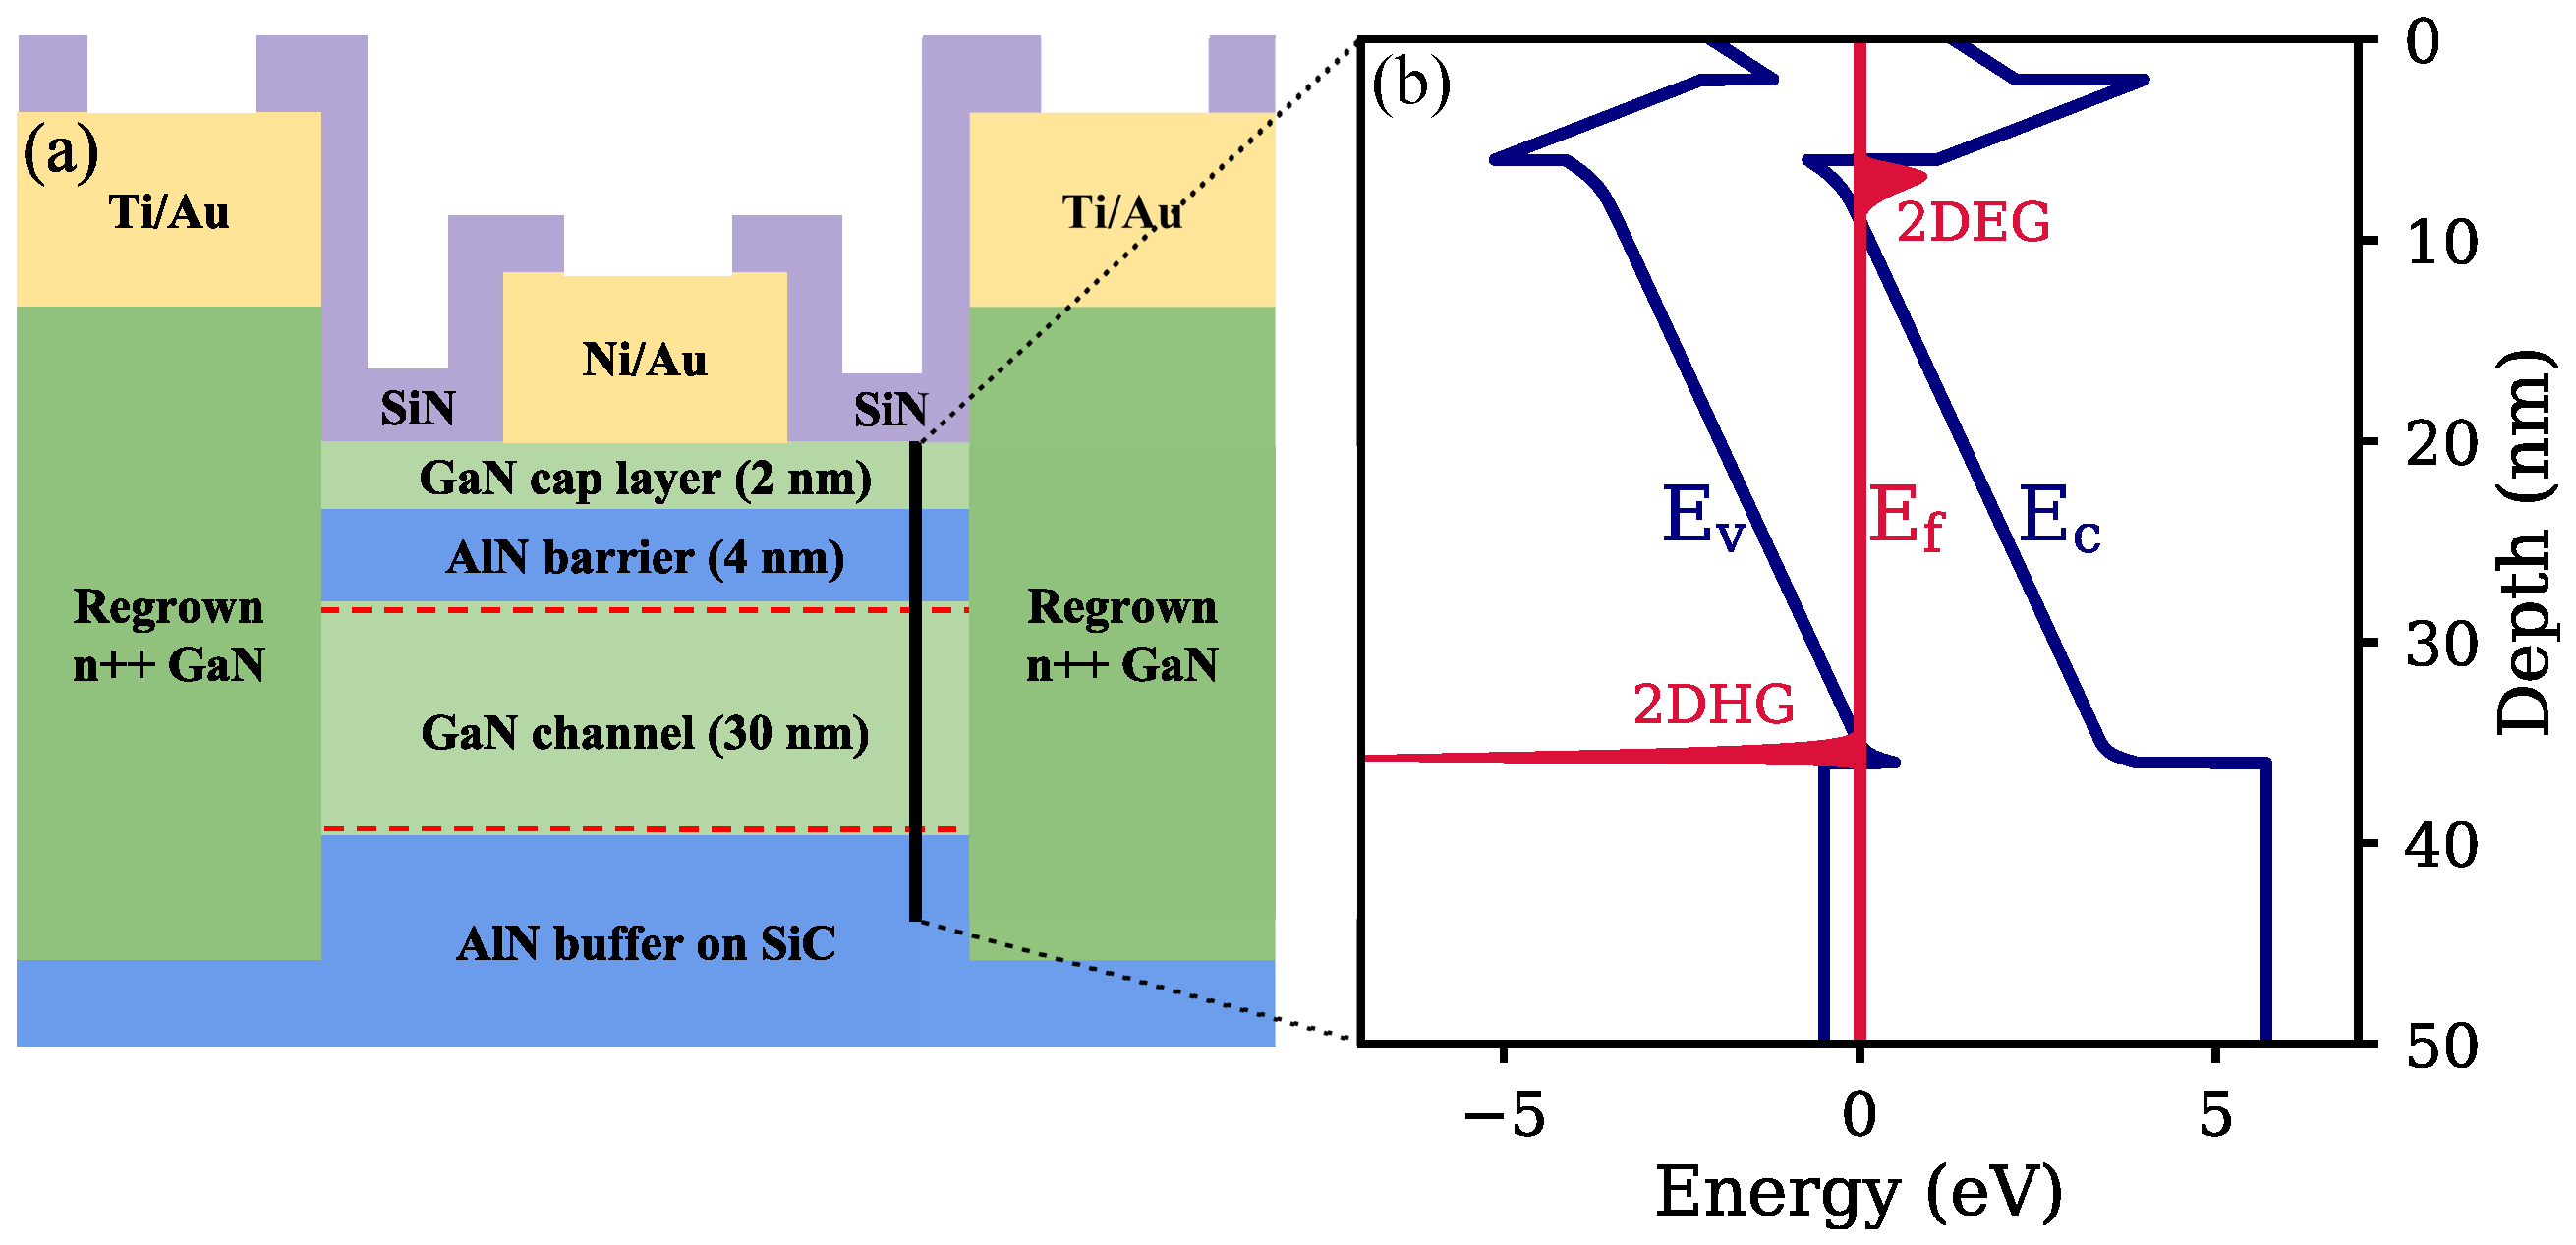
\includegraphics[width=\columnwidth]{Figure1.eps}
\caption{(a) Cross-sectional representation of a processed QW HEMT, and (b) corresponding energy band diagram simulated by 1D Poisson. }
\label{fig:epi}
\end{figure}

\begin{figure*}[!t]
\centering
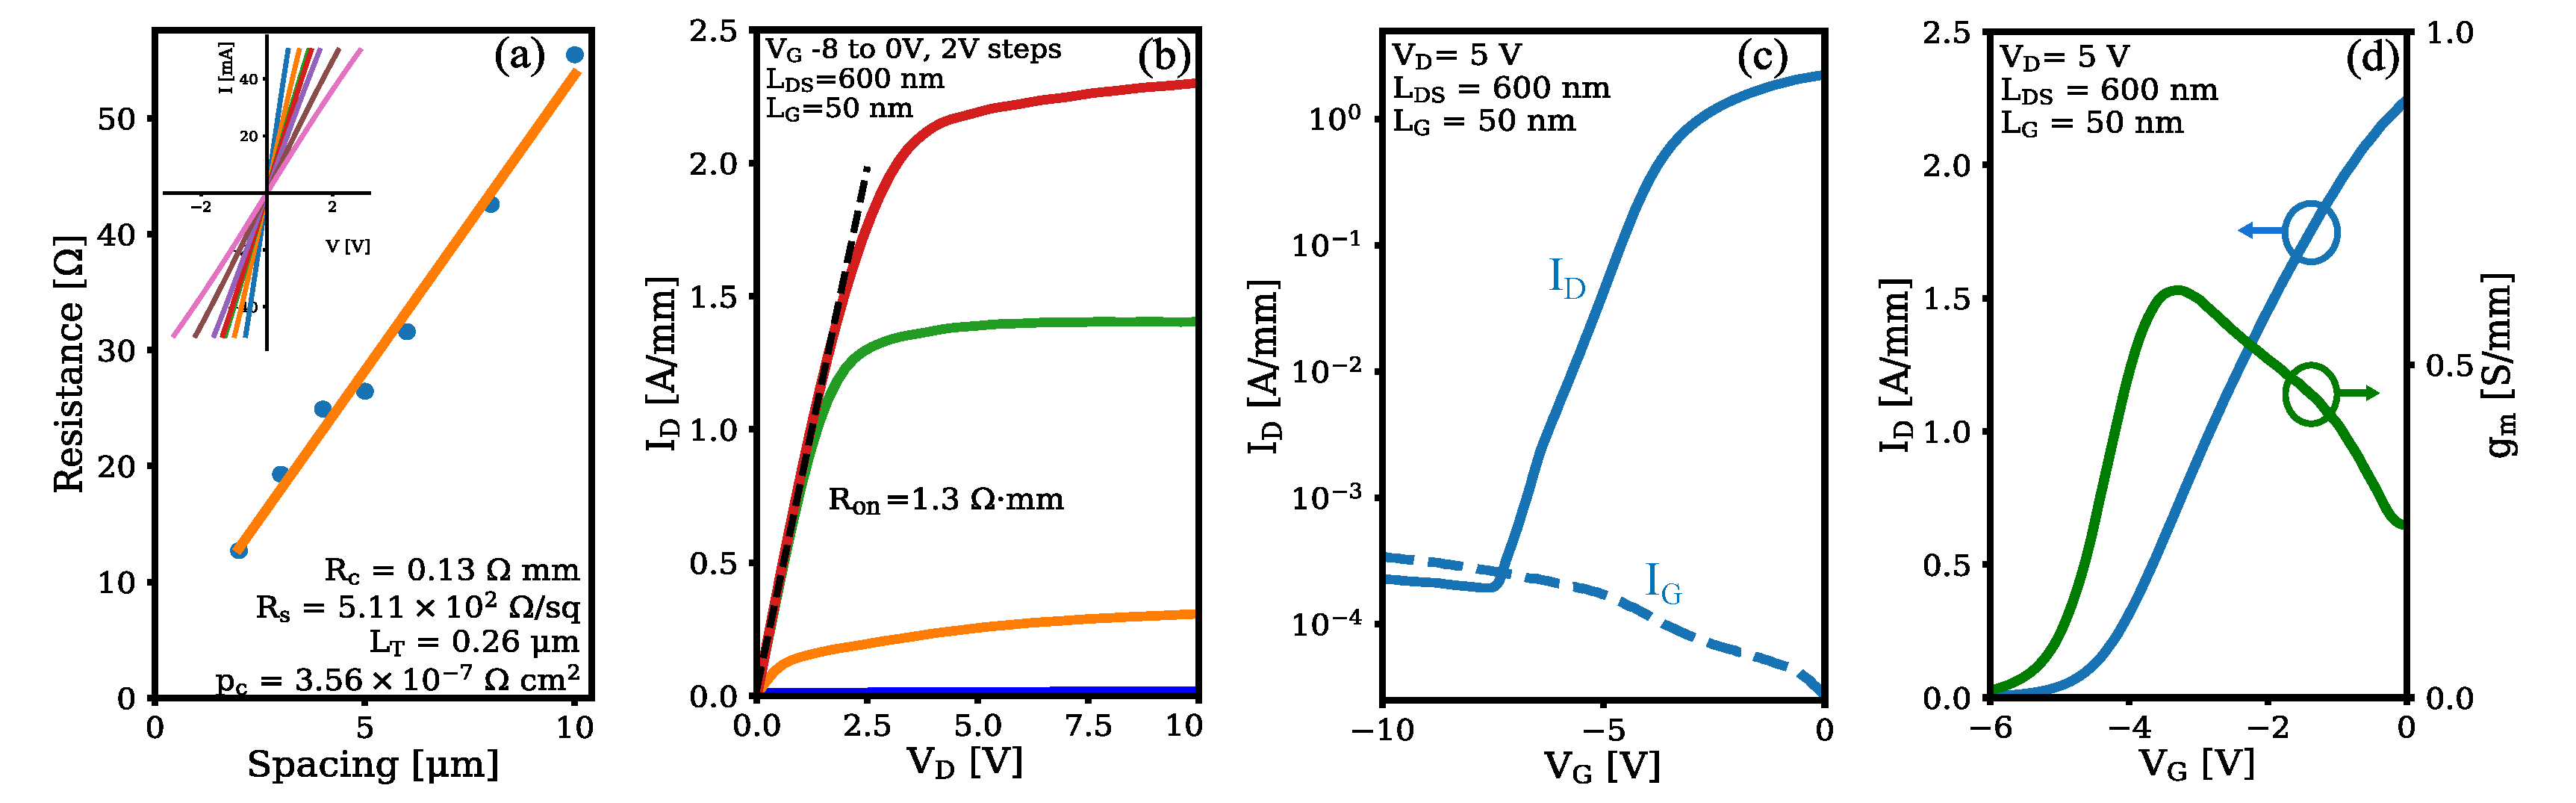
\includegraphics[width=\textwidth]{Figure2.eps}
\caption{(a) Linear TLM analysis of the non-annealed Ti/Au ohmic contacts to the regrown GaN. (b) $\mathrm{I_DV_D}$ curves demonstrating current saturation for $\mathrm{I_D}\sim$2.3 A/mm with low $\mathrm{R_{on}}$ = 1.3 $\Omega\cdot$mm. (c) Log-scale transfer curves showing on/off ratio of $\mathrm{10^4}$ limited by gate leakage current. (d) Linear transfer curves reveal peak $\mathrm{g_m}$ = 0.6 S/mm, the highest transconductance reported for QW HEMTs. }
\label{fig:IdVg}
\end{figure*}

\section{Device Fabrication}
The AlN/GaN/AlN epitaxial structures were grown by plasma-assisted molecular beam epitaxy (MBE) on semi-insulating 6H silicon carbide substrates. The heterostructure consists of a 350 nm AlN buffer layer, a 30 nm GaN channel, a 4 nm AlN barrier, and a 2 nm GaN passivation layer as shown in Fig. 1(a). Room temperature Hall-effect measurements prior to device fabrication showed a two-dimensional electron gas (2DEG) sheet concentration of 2.9 $\cdot$ $\mathrm{10^{13}}$ $\mathrm{cm^{-2}}$ and electron mobility of 630 $\mathrm{cm^2}$/V·s, corresponding to a sheet resistance of 340 $\Omega$/sq.  \textcolor{black}{The highest mobilities reported for the AlN/GaN/AlN heterostructure are currently $\sim$700 $\mathrm{cm^2}$/V·s at room temperature \cite{Wang2012,Islam2016,Song2017,Rennesson2018}. Several factors may be playing a role in the mobility limitation, including the high electron concentration that may increase the electron effective mass, increased interface roughness scattering, and the possibility for a 2D hole gas (2DHG) at the GaN channel/AlN buffer interface. However, a full analysis of the mobility in this heterostrucutre is outside the scope of this report.}

An energy band diagram of the as-grown heterostructure simulated via self-consistent solution of the Poisson and Schrodinger equations \cite{Tan1990} is shown in Fig. 1(b) shows the formation of a 2DEG at the top AlN/GaN heterojunction. The simulation also indicates the formation of a 2DHG at the bottom GaN/AlN heterojunction. The 2DHG has been experimentally detected in the AlN/GaN/AlN heterostructure via terahertz spectroscopy \cite{Jena2017}, \textcolor{black}{and it has been confirmed in an undoped GaN/AlN heterostructure \cite{Chaudhuri2018}. If present in the QW HEMT, the 2DHG may act as a floating body or dynamic field plate, depending on the contact quality. The behavior of the 2DHG merits more detailed studies in the future.}

The device fabrication used a realigned gate-last process. The heterostructure was patterned with a $\mathrm{SiO_2}$/chromium hard mask and etched via $\mathrm{BCl_3}$ inductively coupled plasma (ICP) to expose the 2DEG sidewall. The sample was loaded back into the MBE, and regrown n++ GaN ($\mathrm{N_D}\sim10^{20} \mathrm{cm^{-3}}$) source/drain contacts were formed. The $\mathrm{SiO_2}$/Cr mask was removed via HF, and device isolation was achieved by another $\mathrm{BCl_3}$ ICP etch that extended 20 nm into the AlN buffer. Ti/Au (50/50 nm) non-alloyed ohmic contacts were deposited by e-beam evaporation on top of the regrown GaN source/drain regions. Long-channel gates were patterned by photolithography, and Ni/Au (50/50 nm) Schottky contacts were deposited by e-beam evaporation directly on the sample surface. Submicron channel devices were patterned for RF gates using electron beam lithography (EBL) with a PMMA bilayer. Ni/Au (20/50 nm) Schottky contacts were deposited via e-beam evaporation directly on the sample surface. Gate lengths as short as 40 nm were observed via SEM, shown in Fig. 4(a). No field plate was implemented. The HEMTs were then passivated with low-power, plasma-enhanced chemical vapor deposition (PECVD) silicon nitride with a thickness of 40 nm. Contact holes were formed in the silicon nitride by 6:1 BOE etching to allow probing of the ohmic and gate contact pads. The final HEMT cross-section is shown in Fig. 1(a).

\begin{figure}[!b]
\centering
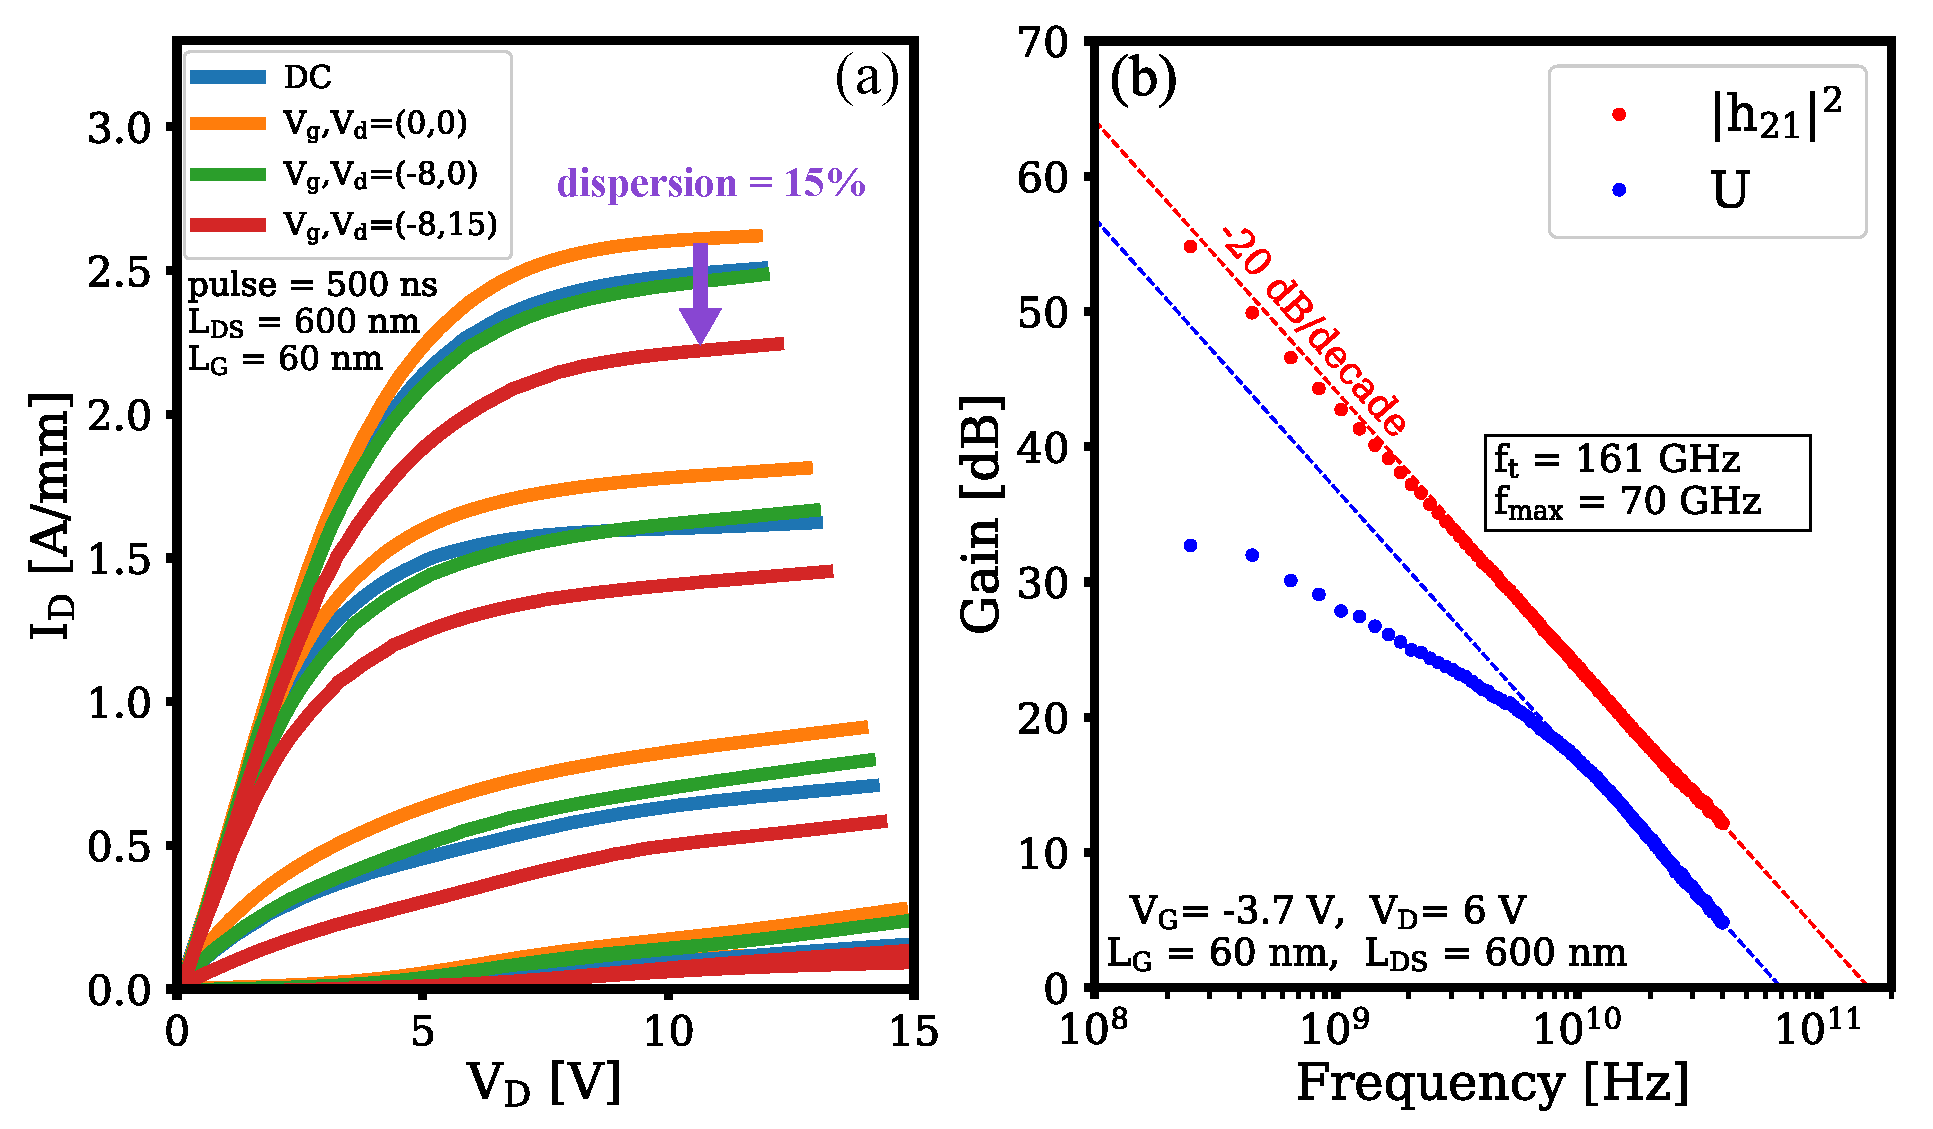
\includegraphics[width=\columnwidth]{Figure3_withsmallsignal.eps}
\caption{\textcolor{red}{(a) Pulsed $\mathrm{I_D-V_{DS}}$ measurements after SiN passivation of a QW HEMT with $\mathrm{L_G}$ = 60 nm, demonstrating moderate dispersion up to 15 V. (b) Small-signal measurements of the passivated QW HEMT with $\mathrm{f_t/f_{max}}$ = 161/70 GHz.}}
\label{fig:pulsed}
\end{figure}


\begin{figure*}[!t]
\centering
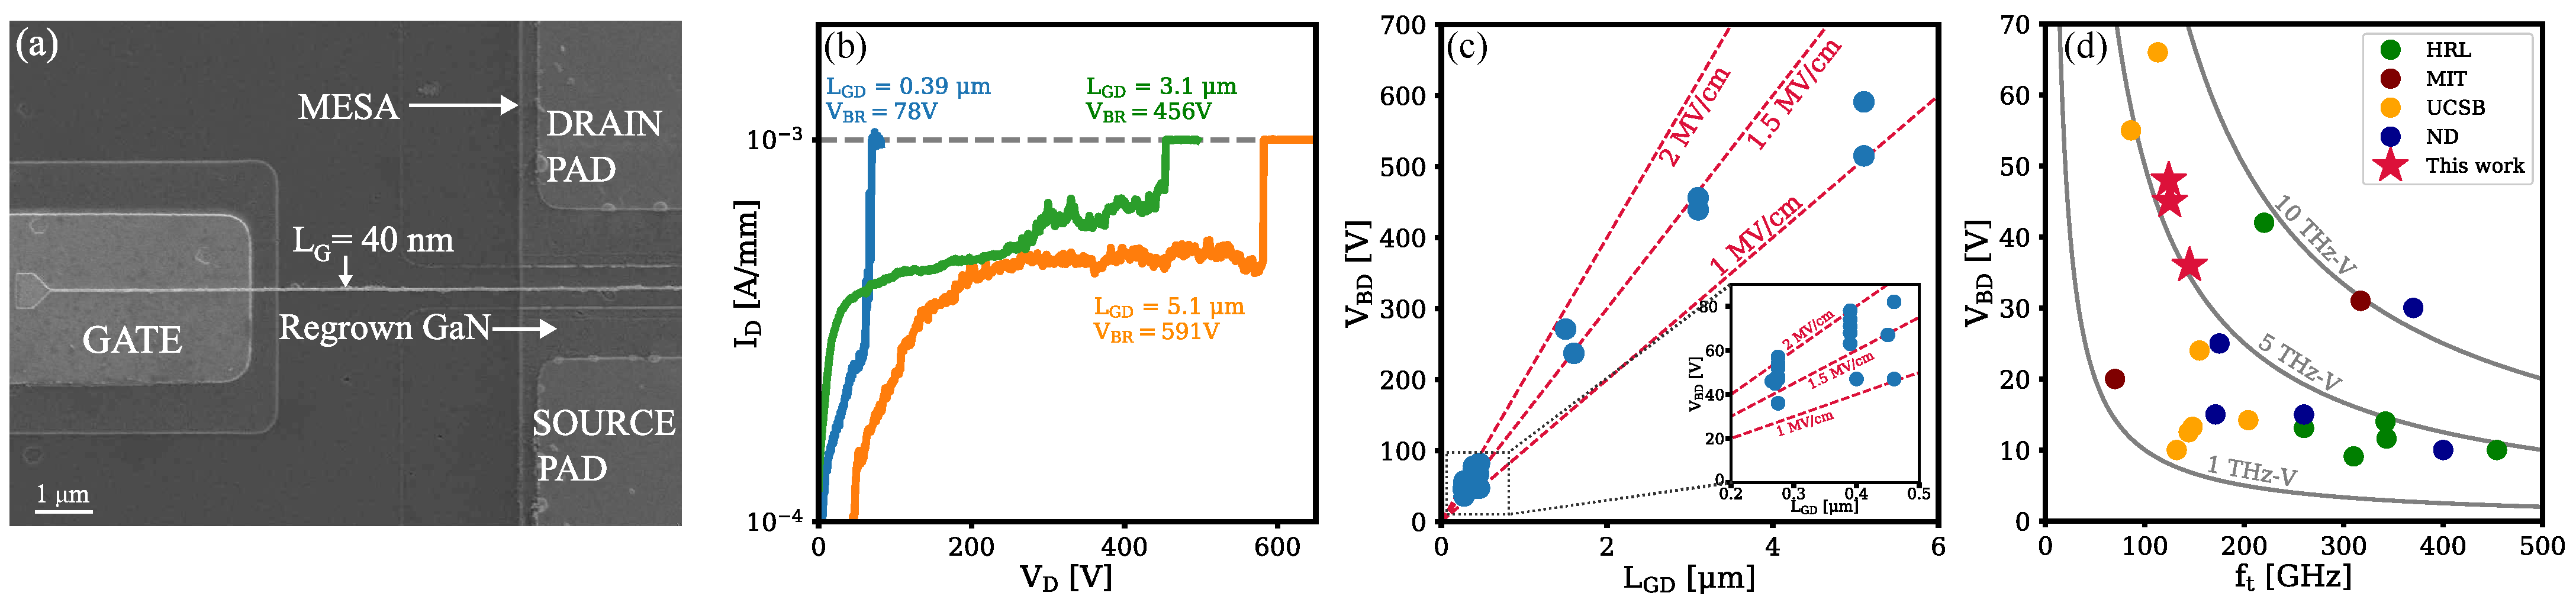
\includegraphics[width=\textwidth]{Figure4_JFoM.eps}
\caption{ (a) SEM image of a short-channel QW HEMT with $\mathrm{L_G}$ = 40 nm. (b) Hard breakdown for three HEMTs with varied gate-drain separations. (c) Breakdown voltage scaling as a function of gate-drain separation ranging from 0.27 to 5.1 $\mu$m. (d) \textcolor{red}{Johnson figure of merit benchmark plot comparing the QW HEMT to state-of-the-art GaN HEMTs with submicron $\mathrm{L_{GD}}$ and no field plate.} }
\label{fig:benchmark}
\end{figure*}

\section{Experimental Results and Discussion}
\label{sec:Experimental Results and Discussion}
After device fabrication, transfer-length method (TLM) patterns were measured in multiple locations across the sample, revealing excellent ohmic contact to the 2DEG with a contact resistance of $\mathrm{R_c}$ = 0.13 $\Omega\cdot$⋅mm, shown in Fig. 2(a). Hall-effect measurements at room temperature after fabrication revealed a 2DEG sheet concentration of 3 $\cdot$ $\mathrm{10^{13}}$ $\mathrm{cm^{-2}}$ and an electron mobility of 410 $\mathrm{cm^2}$/V·s, resulting in a sheet resistance of 510 $\Omega$/sq. The sheet resistance increased 50\% from its as-grown value, likely due to surface damage induced during the fabrication process and could be potentially avoided by changing the $\mathrm{SiO_2}$ deposition process. Transfer I-V characteristics reveal an $\mathrm{I_{on}}/\mathrm{I_{off}}$ = $\mathrm{10^4}$ (this value was $\mathrm{10^9}$ before passivation) with a peak transconductance of 0.6 S/mm, as shown in Fig. 2(c, d). This is the highest transconductance reported for devices on the AlN/GaN/AlN heterostructure platform and shows their high promise. The output characteristics, plotted in Fig. 2(b), show a drain current of $\sim$2.3 A/mm with excellent saturation and on-resistance of 1.3 $\Omega\cdot$mm.

\textcolor{red}{Pulsed $\mathrm{I_D-V_{DS}}$ measurements were performed after silicon nitride passivation to verify dispersion control, shown for a QW HEMT with $\mathrm{L_G}$ = 60 nm in Fig. 3(a). Bias-dependent S-parameters were then measured in the range of 0.05-40 GHz. The system was de-embedded via a short-open-load-through (SOLT) impedance standard substrate and on-wafer open/short structures. The $\mathrm{f_t}$ and $\mathrm{f_{max}}$ values were extracted from $\mathrm{\vert h_{21}\vert^2}$ and unilateral (U) gain plots. The device measured for dispersion also demonstrated $\mathrm{f_t}$ = 161 GHz, $\mathrm{f_{max}}$ = 70 GHz, as shown in Fig. 3(b). Both $\mathrm{f_t}$ and $\mathrm{f_{max}}$ values are records for HEMTs on the AlN platform. Further scaling of gate length and incorporation of a T-gate geometry are expected to dramatically increase $\mathrm{f_t}$ and $\mathrm{f_{max}}$ for the QW HEMT.}

To investigate breakdown characteristics, the gate voltage was set below the threshold voltage (typically $\mathrm{V_G}$ = -8 V), and $\mathrm{V_{DS}}$ was increased until HEMT breakdown occurred. The breakdown voltage metric is defined as $\mathrm{I_D}$ $\geq$ 1 mA/mm. QW HEMTs were tested for gate-drain lengths ($\mathrm{L_{GD}}$) ranging from 270 nm to 5.1 $\mu$m. The devices were covered in Fluorinert during the measurement process.

Fig. 4(b) shows the three terminal off-state breakdown of three QW HEMTs with varied gate-drain distances. Among all devices, the highest breakdown voltage observed is $\mathrm{V_{BD}}$ = 591 V ($\mathrm{L_{GD}}$ = 5.1 $\mu$m), corresponding to an average electric field ($\mathrm{E_{BD}}$) of 1.16 MV/cm. All measured devices had average electric fields above 1 MV/cm at breakdown. During the measurement process and prior to breakdown, the gate current is found to be roughly equal to the drain current. This indicates the off-state drain current and breakdown is dominated by gate-drain leakage and not avalanche or channel breakdown, and is far from the material limits. 
\textcolor{black}{Future breakdown measurements may improve by refining the SiN passivation process to minimize any increase in the gate leakage current.}



To explore the potential for high-frequency applications, submicron channel lengths were examined for breakdown. A breakdown voltage of 78 V was measured for a HEMT with 390 nm gate-drain distance. This corresponds to an effective breakdown field of 2 MV/cm. This is among the largest breakdown voltages reported for a submicron channel nitride HEMT, demonstrating the potential of QW HEMTs for extremely high-power operation in RF applications. Fig. 4(c) shows the scaling of breakdown voltage as a function of $\mathrm{L_{GD}}$. The breakdown voltage does not scale linearly with $\mathrm{L_{GD}}$, which is expected due to the non-uniform distribution of the E-field within the channel.



\section{Conclusions and Benchmarking}
\textcolor{red}{The breakdown voltages and cutoff frequencies measured in this work are benchmarked against state-of-the-art GaN HEMTs with submicron $\mathrm{L_{GD}}$, and no field plate \cite{Shinohara2010,Shinohara2011,Shinohara2011a,Tang2015,Chung2010,Hemts2006,Saunier2012,Snider2012,Guo2013,Lee2013,Dasgupta2009,Nidhi2012,Denninghoff2012,Denninghoff2012a,Denninghoff2013,Romanczyk2018,Shinohara2012,Yue2013} using the Johnson figure of merit (JFoM), as shown in Fig. 4(d). The breakdown voltage for QW HEMTs is among the highest reported for submicron channel devices, and a JFoM of 5.95 THz$\cdot$V is achieved.}

In this letter, the breakdown characteristics of strained AlN/GaN/AlN quantum well HEMTs were explored for the first time. The fabricated devices demonstrated excellent DC characteristics, with $\mathrm{R_c}$ = 0.13 $\Omega\cdot$mm, $\mathrm{I_{Dsat}}$ = 2.3 A/mm, and peak $\mathrm{g_m}$ = 0.6 S/mm. HEMTs with $\mathrm{L_{GD}}$ ranging from 270 nm to 5.1 $\mu$m were tested for breakdown characteristics, and a clear dependence of breakdown voltage on gate-drain distance is observed. \textcolor{red}{Small-signal RF measurements revealed record performance for HEMTs on the AlN platform, with $\mathrm{f_t/f_{max}}$ = 161/70 GHz.} High breakdown voltage is observed across all gate-drain lengths, most notably for submicron channel devices, in which a breakdown voltage of 78 V was measured for a device with $\mathrm{L_{GD}}$ = 390 nm, $\mathrm{L_{SD}}$ = 800 nm. \textcolor{red}{The combination of high breakdown voltage and moderate cutoff frequency demonstrate QW HEMTs as a viable platform and potential successor to AlGaN/GaN HEMTs for future high-power RF electronics.}

\vfill

% Just to move references to the fourth page so it's clear
% that my document ends at 2 2/3 pages
{\color{white}
\pagebreak
}

\bibliographystyle{IEEEtran}
%\bibliography{link}

\bibliography{breakdown_bib}

\end{document}


